\documentclass[notitlepage]{article}

\usepackage{amsfonts}
\usepackage{amssymb}
\usepackage{amsmath}
\usepackage{amsthm}
\usepackage{graphicx}
\usepackage{tikz}
\usetikzlibrary{arrows,automata}
\usepackage{algorithm2e}
\usepackage{algorithmic}
\usepackage{appendix}
\usepackage{hyperref}
\usepackage{datetime}
\usepackage{fancyhdr}
\usepackage{semantic}
\usepackage[noload]{qtree}
\usepackage{comment}
\usepackage{pdflscape}
\usepackage{graphicx}
\usepackage[margin=1in]{geometry}
\usepackage{moreverb}
\usepackage{caption}
\usepackage{url}
\usepackage{layout}
\usepackage[loose]{subfigure}
\usepackage{lineno}
\usepackage{bm}
\usepackage{tabularx}
\usepackage{hhline}

\definecolor{R}{RGB}{220,20,60}

\newcommand{\red}[1]{{\textcolor{R}{#1}}}
\newcommand{\arr}{\mathbb{R}}
\newcommand{\st}{\;\; st \;\;}
\newcommand{\nat}{\mathbb{N}}
\newcommand{\pr}{\mathbb{P}}

%Uncomment this if you're a BOSS
%\usepackage[annatar]{tengwarscript}
%\newcommand{\tengm}{\mbox{\Tmalta}}


\newtheorem{proposition}{Proposition}

\begin{document}

\input{./title.tex}

\newpage

\section{Introduction}

\begin{figure}[h]
\centering
\begin{tabular}{|c|p{9.5cm}|l|}
\hline
{\bf Group Member} & {\bf Contribution Outline} & {\bf Contribution \%} \\
\hhline{|=|=|=|}
tj0824 & Hand-crafted buffer overflow shellcode, researched NX bits, overcame ASLR \& wrote technical details for attacks & A Noble 50\% \\
\hline
do6613 & Explored tools, automated advanced format string attacks \& stopped Tim from writing a small novel for report & A Saintly 50\% \\
\hline
\end{tabular}
\end{figure}

Together, we have exploited a pair of security issues in some very poorly written programs. Being experienced in various
security exploits, we decided to both attempt each task independently, resulting in subtly different attacks, which can
then be compared and contrasted for their various features. Whilst some steps in our attacks our similar or identical,
we did on occasion make effort to differ; using different format specifiers in the first lab, and finding alternative
methods to generate working shellcode in the second. Also of note is that we attacked both SEED virtual machines, for
the sake of completeness.
asdfgh
% For the second attack, we each converged on the same basic solution -- a standard NOP sled comprising a block of
% addresses, a large ``sled" made of around 450 NOP instructions, and a code payload at the very end. Execution was
% diverted to a point in the sled, allowing it to slide down into the payload. Tim's payload was written in x86 assembly
% which was then assembled with gcc and briefly analysed before being placed at the end of the sled. Drum instead used
% Metasploit to generate a payload for him, instructing the generator to launch /bin/sh and avoid null bytes.


\section{Solution}

\subsection{Attack 1, the Format String Vulnerability}

The {\tt printf, fprintf, sprintf}, etc functions in the standard C IO library are all vulnerable to format string based
attacks, which exploit the manner in which C handles calls to the class of functions they belong to: \textbf{variadic
functions}\cite{vfunc}. When a function is called in the C programming language,\cite{call_conv} the exact actions are
dependent on the specific processor architecture, compiler and operating system. In the case of the lab machines, the
situation is similar to that depicted in figure \ref{fig_stack}.

\begin{figure}[ht] \centering 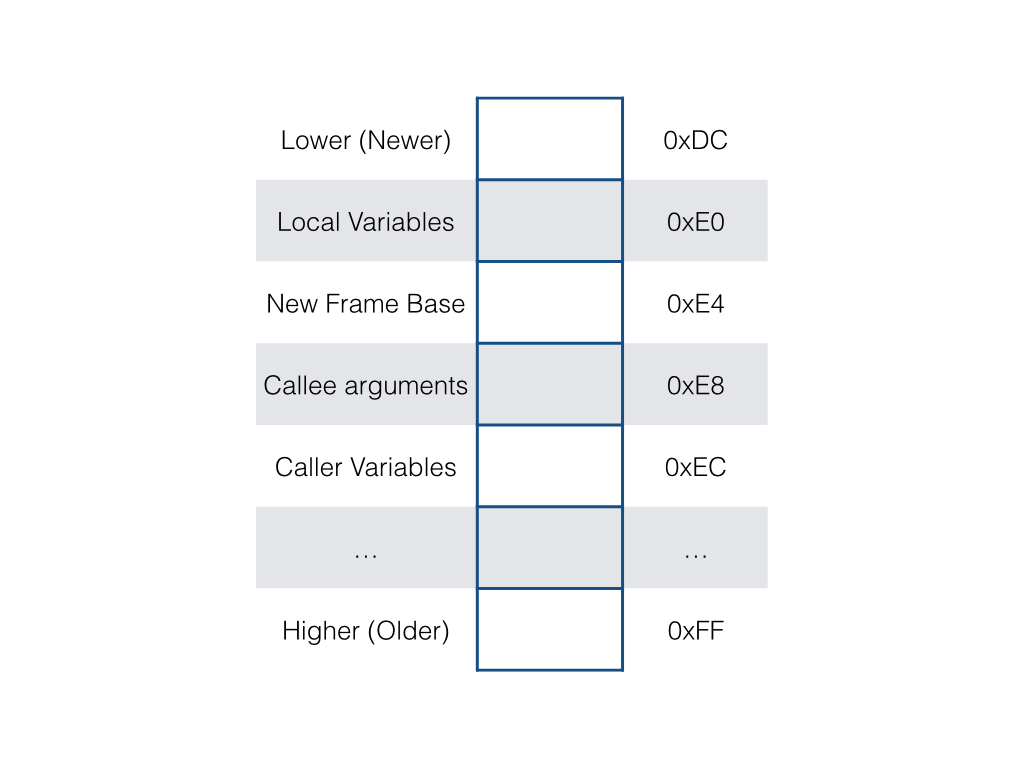
\includegraphics[width = 0.65\textwidth]{./images/stack.jpg} \caption{An example stack,
showing the dangerous arrangement of a function's arguments and its caller's local variables} \label{fig_stack}
\end{figure}

Format string functions are useful and powerful, but can be dangerous; Their intended use is along the line of {\tt
printf("\%x", x)} which prints the value of the variable {\tt x} interpreted as a hexadecimal integer. However, {\tt
printf} blindly trusts the format string to reflect the arguments. {\tt printf("\%x \%x \%x")} will print outthe values
of whatever is stored at the memory locations where the $2^{nd}$, $3^{rd}$ and $4^{th}$ arguments to printf should be if
they existed, without checking whether they exist or not. This means just using format specifiers we can start reading
memory from the stack that doesn't belong in the current context. If, then, we call {\tt printf("\%s\%s...\%s")}, the
program will tear values from the stack, interpret them as memory addresses that contain null-terminated strings, and
attempt to deference and print them. This will segfault quickly as the program attempts to access unauthorised
addresses. Similarly {\tt printf("\%n\%n...\%n")} will tear addresses from the stack, dereference them, set those
locations to 0x0, and again crash when it hits an invalid address.

With the version of the program that requested an integer input, both our attacks used that input as the target address.
In the subsequent version we both used the format string itself to determine where to write. In the first case, we simply supply the appropriate address in integer form, converted from the output printed by the program. This location is equivalent (when stack protectors are disabled) to where the 9th 4-byte argument to a printf call would sit. Thus {\tt printf("\%8x\%8x\%8x\%8x\%8x\%8x\%8x\%8x\%n")} will dig eight words from the stack to
the integer input by the user, then set the value at that memory address to 64 = 0x40. Using another {\tt\%x} would read
the data. You can also leverage positional argument syntax to directly investigate the stack without changing it, which
Drum chose to implement in all of his attacks. Using that syntax, reading the ninth integer would look like this: {\tt
printf("\%9\$8x")}, and writing to it would be {\tt printf("\%9\$n")}.

Setting the address to large values like {\tt 0xd09f00d} can be very difficult, since this requires an
exceptionally long string.

Both of our memory alteration attacks use the {\tt \%n} format specifier to write to an arbitrary value to the memory
address of {\tt secret[1]}. For contrast we decided to use alternate methods of padding the format string to the correct
byte length.

Drum's attack used a padding specifier to an unsigned integer format specifier, or omitted the string entirely, which
allows for the writing of values less than the printed length of the smallest stack variable. Writing a value of 0 to
{\tt secret[1]} without using this method and positional arguments is impossible. Tim's attack uses the more
tried-and-tested approach of standard stack popping, meaning that the minimum writeable value is determined by the
values in the stack and the width specifiers used when they are printed.

\subsection{Attack 2, riding the NOP Sled}

The exploit we used is based on the standard NOP sled and stack smashing approach, where we clobber the stack in order
to manipulate the return address of the current function. If the return pointer can be rewritten to point to the start
of the bytecode provided in the lab, then the running program will execute the bytecode and turn itself into a shell.
Unsafe string functions such as {\tt strcpy} will write strings past the end of their buffer, if not terminated,
regardless of how wide the buffer actually is. By writing a sufficiently long string, we can overflow the buffer and
overwrite memory lower down (higher memory addresses) on the stack, such as the return pointer.

Precisely engineering the return pointer to point exactly to the shellcode's location is often difficult. Though this
would be possible in this example without memory randomization, where we have GDB and access to the source code, when
memory address randomization is enabled it still becomes very difficult. We need extra flexibility a NOP sled provides
it. We construct our sled generally as follows:

An address which is somewhere earlier in the stack than the start of the current frame's return pointer is repeated
(endian-ness accounted for, avoiding null bytes) several times until it would clobber the return address. Then a large
series of no-operation instructions in precompiled bytecode is prepended to the shellcode, and this new blob is appended
to the repeated addresses. Jumping the execution into any one of those NOPs will cause the program to slide down its own
stack directly into the shellcode payload, making memory addresses much easier to guess.

In order to ensure that the resulting shell is indeed a root shell, we need to invoke a {\tt setuid} before launching a
shell. There are a few ways to make this modification to the shellcode -- Tim chose to copy the assembly code from the
assignment sheet, and add some extra lines to make this call. {\tt xorl \%ebx \%ebx} will set the general-purpose
register {\tt \%ebx} to 0. {\tt lea 0x17(\%ebx) \%eax} is designed for computing memory addresses, but here we use it to
add {\tt 0x17} to {\tt \%ebx} and store the result in {\tt \%eax}. {\tt int \$0x80} triggers interrupt {\tt 0x80}, a
syscall interrupt. Syscalls are parametrised exclusively by registers\cite{syscalls}. The first parameter is {\tt \%eax
= 0x17}, and tells the kernel to execute {\tt syscall[0x17]}, namely {\tt setuid}. The second is {\tt \%ebx = 0x0},
which is passed as a parameter into {\tt setuid}. {\tt setuid(0)} sets the user id to 0, more commonly known as {\tt
root}. When this call is placed before the code to launch a shell, the shell will be launched with root privileges.
Assembling this and skimming over the bytecode, we find that prepending the payload with {\tt 0x31db8d4317cd80} will get
the job done. Drum simply chose to delegate all shellcode generation to the metasploit framework, replacing the given
shellcode entirely.


\section{Reflection}

\subsection{Causes and Preventative Measures} Both attacks are entirely preventable, with remedies being extremely
simple and indeed automatic in new cases. In the case of format string vulnerabilities, the entire issue can be avoided
by not using user-provided content in any part of the format string. If this is required for some unknown reason, then
careful parsing of the string  is needed beforehand, to guard against improper specifier usage. Tools such as {\tt
splint} can detect  this problem in a codebase\cite{splint_art}, and requiring programmers to pass static analysis will
prevent most, if not all, occurrences. We believe that the main reason this class of vulnerability exists is poor or lazy
coding, and cracking down on that is the best method of prevention. The complexity of patching this problem can vary,
but the detection is straightforward and automatic.

Similarly, in new code, buffer overflow situations can be easily avoided. They occur only where functions that ignore
buffer sizes are used, and for almost all of these functions there are safe alternatives. Again, linter tools can detect
many instances of this vulnerability, meaning that existing codebases in low-level languages can be patched. Preventing
code from offering opportunities for buffer overflows at the compilation stage is now quite easy; stack protectors
(also called canaries) are now compiled in automatically by default, and provide a very effective method of detecting
stack smashing at the point of a function returning. If a smash is detected, then the program crashes. Later versions of
the C standard library and compilers also include a macro definition called {\tt FORTIFY\_SOURCE}, which will attempt to
automagically replace unsafe functions (such as {\tt strcpy}) with safer variants, such as  (such as {\tt
strncpy})\cite{fort_source}. Microsoft also provide a header file, {\tt banned.h}, which will cause usage of unsafe
functions to throw compile time warnings\cite{banned}.

We believe that lazy design is still a problem, but modern compilation toolchains provide excellent safeguards against
casual mistakes which would have previously been highly dangerous. Further enhancements include ASLR (address space
layout randomisation) and NX (non-executable) regions; they make placing code that can be executed much harder, and are
enabled by default in modern operating systems and development toolchains\cite{wiki_aslr,wiki_nx}. It is
interesting to note are that ASLR was added slowly in small steps to various systems, meaning that it didn't mitigate
all attacks straight away. It is entirely software based, unlike NX regions, which require hardware support. Furthermore
it seems that whilst Ubuntu 9.11 upwards, with the i386 architecture, should have an emulation of NX regions enabled by
default\cite{nx_bit}, the SEED virtual machines seem to have disabled them.  Presumably this was for the educational
purposes of these labs.

The common NOP sled is quite detectable in principle, so emulated execution of a program can use simple heuristics to
determine if a basic sled is being deployed. Very few programs would have a legitimate reason for using multiple
consecutive NOPS\cite{zip_quine}, and we believe that is why Metasploit uses a method of generating a NOP sled that
doesn't use NOP instructions, instead using regular instructions in a way that has no side-effects and does no practical
work\cite{wiki_sled}.

All that aside, we believe the best defense is simply to educate programmers about the dangers of their software being
attacked, and how they can design against it.

\subsection{Damage Potential}

By itself, a format string vulnerability offers only limited opportunity for control flow modification, and typically
relies on altering memory locations to affect the vulnerable program rather than hijacking the process completely.
It is, however, possible to create detailed stack dumps, and thus the vulnerability can often serve to
enhance knowledge of the system. This knowledge can then be leveraged in other attacks -- for example, if this
vulnerability exists alongside a buffer overflow, then the damage potential is significantly greater. In most
situations, the presence of a stack canary nullifies the risk of a buffer overflow attack. Using a format string
vulnerability it is possible that an adversary could tear values from the stack in seach of this canary, and duplicate
it at the start of their NOP sled.



\section{Conclusion}

To conclude, both programs are very faulty. Whilst the format string vulnerability doesn't cause major issues in
isolation, the buffer overflow attack allows any user to gain root access to the system, which is a very serious
problem. A format string vulnerability can, however, be used to nullify certain countermeasures against buffer
overflows. The security flaws exposed here are caused by problems which good programming practice can completely
prevent, but which still exist in real-world scenarios to this day. Though few new systems will be subject to these
flaws, the cost of rebuilding a pre-existing system which already exhibits these flaws can be prohibitively high. For
this reason, new programs should be built with security as a priority and thoroughly checked prior to deployment so a
user needn't pay the excessive costs associated with a security breach.


\bibliography{bibliography}{}
\bibliographystyle{plain}

\end{document}
